\section{Relevant Knowledge and Problem Formulation}
\label{sec:relevant-knowledge}
%% Describe relevant orbital parameters - eccentricity, true anomaly, the relation between true anomaly and time, and drag coefficients
The translational dynamics of the chaser are considered to be in the local-vertical-local-horizontal (LVLH) frame of reference of the target.
As depicted in Figure \ref{fig:lvlh_frame}, this reference frame is centered at the center of mass of the target and fixed with respect to the orbit with its Y-axis pointing radially into the center of the Earth, the X-axis pointing opposite to the direction of the velocity of the target spacecraft, and the Z axis pointing along the angular momentum vector of the target, hence completing a right-handed system.
\begin{figure}[htb]
    \centering
    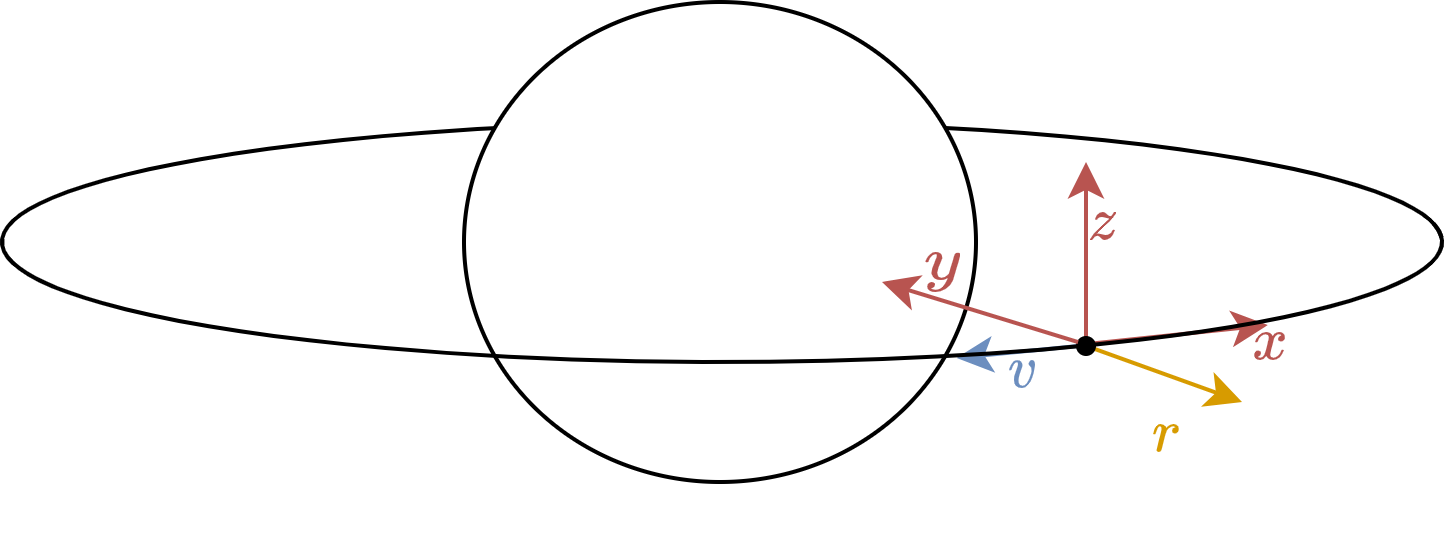
\includegraphics[width=0.9\linewidth]{assets/lvlh_frame.png}
    \caption{Local-Vertical-Local-Horizontal (LVLH) Frame of Reference of the Target}
    \label{fig:lvlh_frame}
\end{figure}
If we assume the orbits of the target and the chaser to be circular, within close proximity to the target, the translational dynamics of the chaser follow the Clohessy-Wiltshire-Hill (CWH) equations (refer to Appendix \ref{app:cwh-equations}).
However, in this paper, we generalize the problem to targets that may be in elliptical orbits around the Earth.
Appendix \ref{app:ellp-undrag} describes the dynamics of relative motion in an elliptical orbit where the chaser and the target may have unequal drag constants.
As considered in the paper, we assume an inverse law, $g(R)=1/R$, to model the variation in atmospheric density.
However, we realize that this inverse law does not perfectly represent the scale of the trend of atmospheric density \cite{emmert2021nrlmsis}.
As a result, we consider the corresponding ratio in variation into the drag constants $\alpha$ (of the target) and $\beta$ (of the chaser).
Such a system considers the true anomaly $\theta$ of the orbit as the independent variable, hence giving the following dynamical equations:
\begin{subequations}\label{second:main}
\begin{align}
    \boldsymbol{r}'(\theta)&=A(\theta,\theta_0)\boldsymbol{r}(\theta)+B\boldsymbol{u}(\theta)+\boldsymbol{d}(\theta, \theta_0)\tag{\ref{second:main}}\\
    \text{where }\boldsymbol{r}(\theta)&=\begin{bmatrix}
    x(\theta),y(\theta),z(\theta),x'(\theta),y'(\theta),z'(\theta)
    \end{bmatrix}^T,\\
    \boldsymbol{u}(\theta)&=\begin{bmatrix}
    u_x(\theta),u_y(\theta),u_z(\theta)
    \end{bmatrix}^T
\end{align}
\end{subequations}
As a result, we will consider true anomaly to be the primary independent variable throughout this paper.
The relation between the true anomaly of the target and the time lapsed since periapsis $t=t_{\text{curr}}-t_p$ is given as:
\begin{subequations}
\begin{align}
    M&=M_0+2\pi\frac{t}{T}\\
    M&=E-{\mathsf{e}}\sin(E)\\
    \theta&=E+2\arctan\left(\frac{\beta\sin(E)}{1-\beta\cos(E)}\right)\\
    \beta&=\frac{{\mathsf{e}}}{1+\sqrt{1-{\mathsf{e}}^2}}
\end{align}
\end{subequations}
where $M$ is the mean anomaly of the target, $E$ is the eccentric anomaly of the target, and ${\mathsf{e}}$ is the eccentricity of the orbit of the target.
Hence, the true anomaly of the orbit can be numerically computed from time and time can be analytically computed from true anomaly.\\
% To follow consistent nomenclature, we use $\theta$ in this paper to represent the true anomaly of the chaser-target system and $\boldsymbol{\theta}$ to represent the angular position of the target.\\
Based on the given information above and the need for reliable solutions to the detumbling problem in orbit, we propose the application of adaptive dynamic tube model predictive control (ADTMPC) to facilitate chaser trajectory planning for rendezvous and docking.
Section \ref{sec:chaser_ampc} deals with the basic trajectory optimization problem followed by the estimation of unknown parameters using adaptive control techniques.
Section \ref{sec:constraints} elaborates on the constraints and bounds involved in this problem. 
This is followed by an explanation of the effects of using dynamic tubes to avoid constraint violation in Section \ref{sec:dynamic-tube}.
Section \ref{sec:multi-agent} proposes techniques to expand this problem using multiple chasers.
The chaser, following its attachment onto the target, needs to exert torque on the target to stop detumbling.
This is discussed in Section \ref{sec:target-deflection}.
We also demonstrate the effectiveness of using ADTMPC over other techniques that do not include elements of this algorithm.
Finally, the appendices provide more information on the dynamics of the chaser for a simplistic (circular orbit with no drag) scenario followed by a more realistic (elliptical orbit with quadratic drag) one.